\documentclass{article}

\usepackage{indentfirst}
\usepackage{graphicx}
\usepackage{wrapfig}
\usepackage{setspace}
\usepackage{url}
\usepackage{pdfpages}

\begin{document}

	\begin{titlepage}
		\vspace*{\fill}
		\begin{center}
			\huge{A Predictive Model of Trees in a Forest using Decision Trees} \\
			\vspace{3cm}
			
			\large{Lucas Kushner} \\
			\vspace{10px}
			\normalsize{\today}		
		\end{center}
		\vspace*{\fill}
	\end{titlepage}	
	
	\doublespacing		
	
	\tableofcontents
	
	\clearpage
	\setcounter{page}{1}
	
	\section{Introduction}
	In this paper, we will be looking at making predictions from a dataset of trees in a forest. Underlying the realistic problem of forest cover-type prediction is a machine learning classification problem. There are many approaches to these types of problems, including perceptron, probabilistic analysis, and decision trees. In this paper, we will explore the last of these options.
	
	\section{Description of Data Set}
	The data set used contains 54 different features for 30 x 30 meter plots of forest. The data was acquired by the United States Forest Service, and a total of 581012 samples were taken. Among these features are geographical characteristics such as elevation, slope, aspect and proximity to water, as well as characteristics of the surrounding soil. Varying numbers of these features were used as the inputs. The type of tree cover in the area was used as the output to be predicted. The full data and description is avaialable at: 
	
	\begin{center} \url{http://kdd.ics.uci.edu/databases/covertype/covertype.html} \end{center}
	
	For the model described in this paper only a small subset of the avaialable data was used, usually with numbers of data ranging in the hundreds or thousands. However, the full dataset contains tens of thousands of data. The data used in this paper were taken from the beginning of the data file, reading the first set of data to be for training, and the second set for testing.
	
	\clearpage
	\section{Description of Algorithm}
	
	\subsection{Decision Trees}
	In approaching this classification problem, we will use a variation of a decision tree. The idea behind the decision tree algorithm is that after constructing a tree which connects the various features of the input vector, we can follow the edge corresponding to the value of that feature. How the edge corresponds to a certain value for a feature is left up to the specific implementation. Once this has been accomplished the process continues, traversing down the tree until a leaf node is reached. The value of this leaf node corresponds to the output predicted by the algorithm. An example of a very simple decision tree is shown below.
	
	\begin{figure}[h]
		\centering
		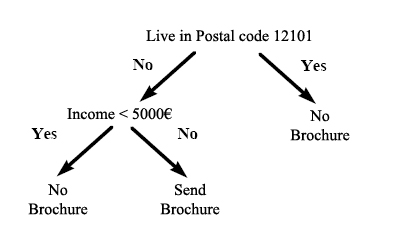
\includegraphics[height=6.5cm]{basic-tree.jpg}
		\caption{An example of a simple, binary decision tree. This tree has strictly "Yes" or "No" values along each of its edges, with the potential outputs shown at the leaf nodes.}
	\end{figure}
	
	\clearpage
	\subsection{Our Decision Tree}
	In the tree used to approach our data set, each edge will have a certain range associated with it. Then, if the value of the feature at a given node falls into this range, we will follow that edge to the next node. We refer to these ranges as the "bins" of the feature. Furthermore, each level of the decision tree will contain nodes which refer to the same feature of the input vector. Even if there are many nodes on the same level of the tree, each node will represent the same feature and have the same number of edges with the same values leading to its children.
	
	\subsection{Bins}
	One charactierstic of our tree which must be determined is the number and sizes of the bins to use for each feature. In this paper, we have chosen to use a pre-determined number of bins. Each feature will have the same number of bins, and the ranges of the bins will be even portions of the total range of the data for that feature. In the case where there are more bins created than there are values in the range of the input (ie. if the feature ranges from 10 - 20 and we have made 15 bins) than additional bins will still be made, even though no values will ever fall into their range.

	\subsection{Entropy}
	Next, we must determine which features of the data we will placed in which levels of the tree. This is done using a feature known as entropy. Entropy is a probabilistic measure of uncertainty in a system. The mathematical definition of entropy is given below.

	\begin{equation} E = -p * log_{2}(p) \end{equation}

	\indent To determine which feature to use, we will calculate the entropy of each feature for the given set of training data, and use those features with the highest entropy closer to the root of the tree. The steps for calculating the entropy of a given feature are as follows:

	\begin{enumerate}
		\item Create the bins for the given feature.
		\item Determine the probability of a given value of that feature falling into a particular bin for each of the bins.
		\item Calculate the entropy of each of these probabilities and sum them.
	\end{enumerate}

	\subsection{Creating and Training the Tree}
	To create the decision tree, we begin by creating a one node tree using the feature with the highest entropy. Then, we give this node the same number of children as bins it has, which each child being of the feature with the second highest entropy. This process is continued recursively for all of the feature of the input vector. An example of what a tree created by this method is shown on the following page.

	The next step is to feed the training data into the decision tree to be placed. During the training phase, each vector of data in the training set trickles down the decision tree until it reaches its appropriate leaf node. Then, the value of that node is overwritten to match the target value of the data vector that was just fed through the tree.
	
	\begin{figure}[h]
		\centerline{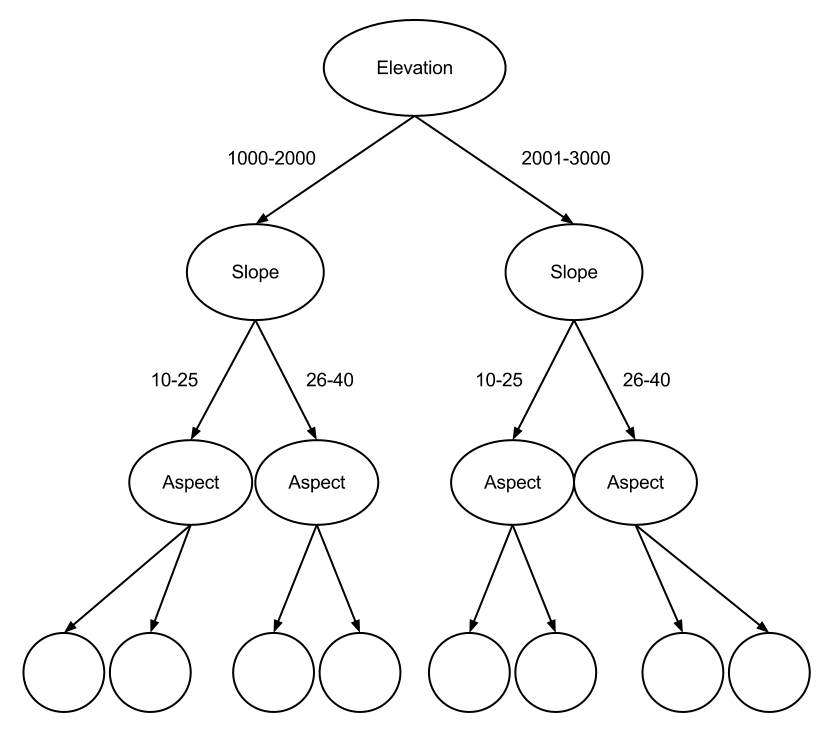
\includegraphics[height=6.5in]{decision-tree.png}}
		\caption{An example of the type of decision tree that will be used in our model.}
	\end{figure}
	
	\clearpage
	
	\section{Results}
	To test the accuracy of this machine learning algorithm, we change one if the characteristics of the tree while holding the rest constant. This was done for the number of bins per feature, the number of features used in the input vector, and the number of training data used to train the tree. In all of these cases, the number of data used for testing was held at a constant number of 500. The graphical results of running these tests is shown below.
	\vspace{3cm}
	
	\begin{figure}[h]
		\centerline{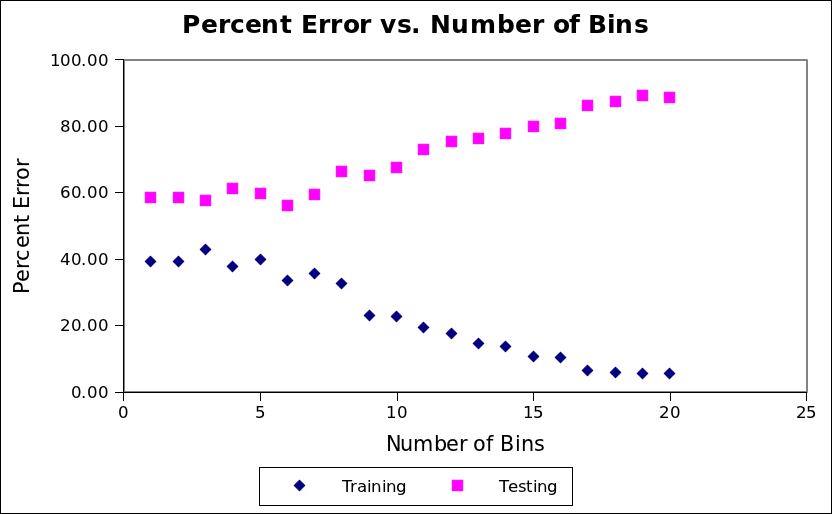
\includegraphics[width = 5in]{bins.png}}
		\caption{The percentage of error versus the number of bins per feature. For these tests, there were 3 features and 800 data used for training.}		
	\end{figure}
	
	\begin{figure}
		\centerline{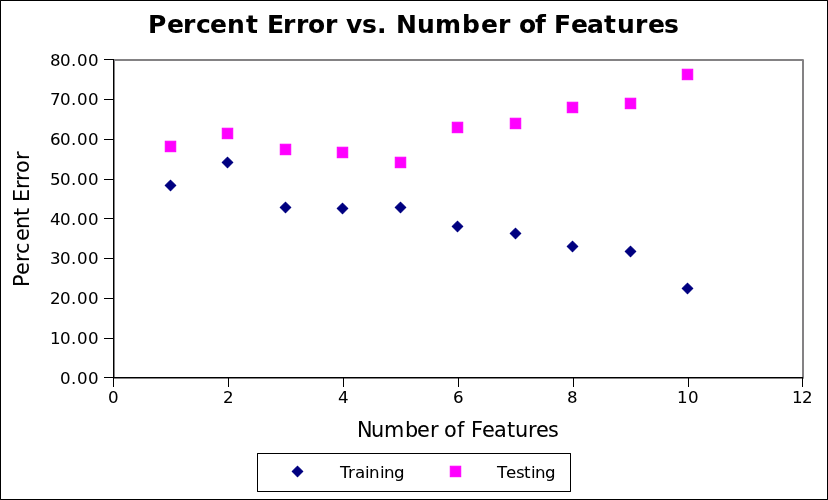
\includegraphics[width = 5in]{features.png}}
		\caption{The percentage of error versus the number of features in the input vector. For these tests, there were 3 bins per feature and 800 data used for training.}		
	\end{figure}
	
	\begin{figure}
		\centerline{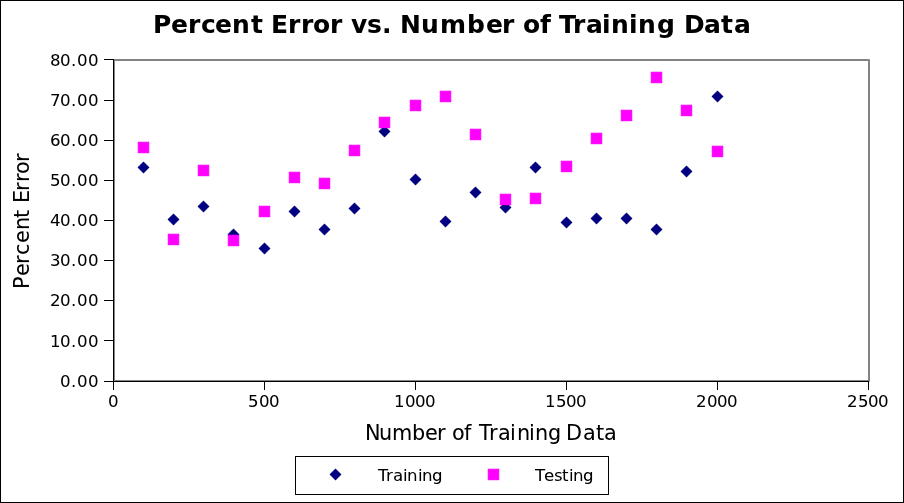
\includegraphics[width = 5in]{training.png}}
		\caption{The percentage of error versus the number of training data used to train the tree. For these tests, there were 3 features and 3 bins per features used.}		
	\end{figure}
	
	\section{Anlaysis of Results}
	The results shown above lead to some interesting conclusions about this particular decision tree algorithm. Firstly, Figures 2 and 3 clearly demonstrate that as the accuracy in validation the training data increases, the accuracy of prediction the testing data decreases. This inverse relationship is indicative of a tree which is overfitted to the training data. As we increase the number of bins and features, the tree becomes increasingly large, the number of leaf nodes increase, and therefore there is a finer resolution on matching a predicted output to a given input vector. However, this also means that the tree start becoming custom-tailored to the given training set, and not general enough to handle new inputs.
	
	Although it is less clear, Figure 4 also shows signs of overfitting data. Despite the lack of immidiately distinguishable pattern in the graph, note that as the error in predicting the training set decreases, the error in prediction of the testing set increases. This pattern matches the relationships displayed in Figures 2 and 3, again hinting at possible overfitting in the tree.
	
	Regardless of the issue of overfitting, the tree was very inaccurate in making predictions about the testing data. At its best conditions for the various tests run, the smallest amount of error in its predictions was 35\%, with percentages as high as 89\% in cases of substantial overfiting.
	
	\clearpage
	\section{Potential Improvements}	
	\subsection{Range Determination}
	There are various improvements that could be made to the described decision tree algorithm in order to improve its performance. Perhaps the most intuitive improvement would be to ensure that all features values of the test data will fall into the range of the training data. In our model, there is no explicit check to ensure that all of the test data will be able to properly traverse the tree. There is a possiblity that the value of some feature in the test data may not fall into any of the bins for that feature in the tree. When this occurs, it is interpreted as an incorrect prediction, so elimination this possiblity may increase the accuracy of predictions. Furthermore, splitting ranges based on probability instead of raw values may improve accuaracy as well. For example, if instead of splitting ranges to contain 1/4 of the possible values they were split so any data had a 25\% chance of falling into each range, then the distribution of data when training the tree would be more even, decreasing the number of conflicting outputs at a given leaf node.
	
	\subsection{Probabilistic Training}
	Additionally, finer control of training in the tree may also increase the accuracy. Currently, if a training data ends up reaching a leaf node which already has a value stored in it, then the existing value is simply overwritten. If instead one were to keep track of all of the expected outputs which corresponded to a given leaf node and assign the most probable of these as the predicted output for that node, then the value will more accurately reflect the training data.
	
	\clearpage
	\section{Conclusion}
	Overall, the model proposed in this paper is not particularly good at making predictions on the given data set. It shows significant signs of readily overfitting to the training data, and is not particularly accurate of whether overfitting has occurred. However, if some of the improvements mentioned were to be implemented, then it is likely that the accuracy of the resulting decision tree could produce a viable, predictive model of the data.

	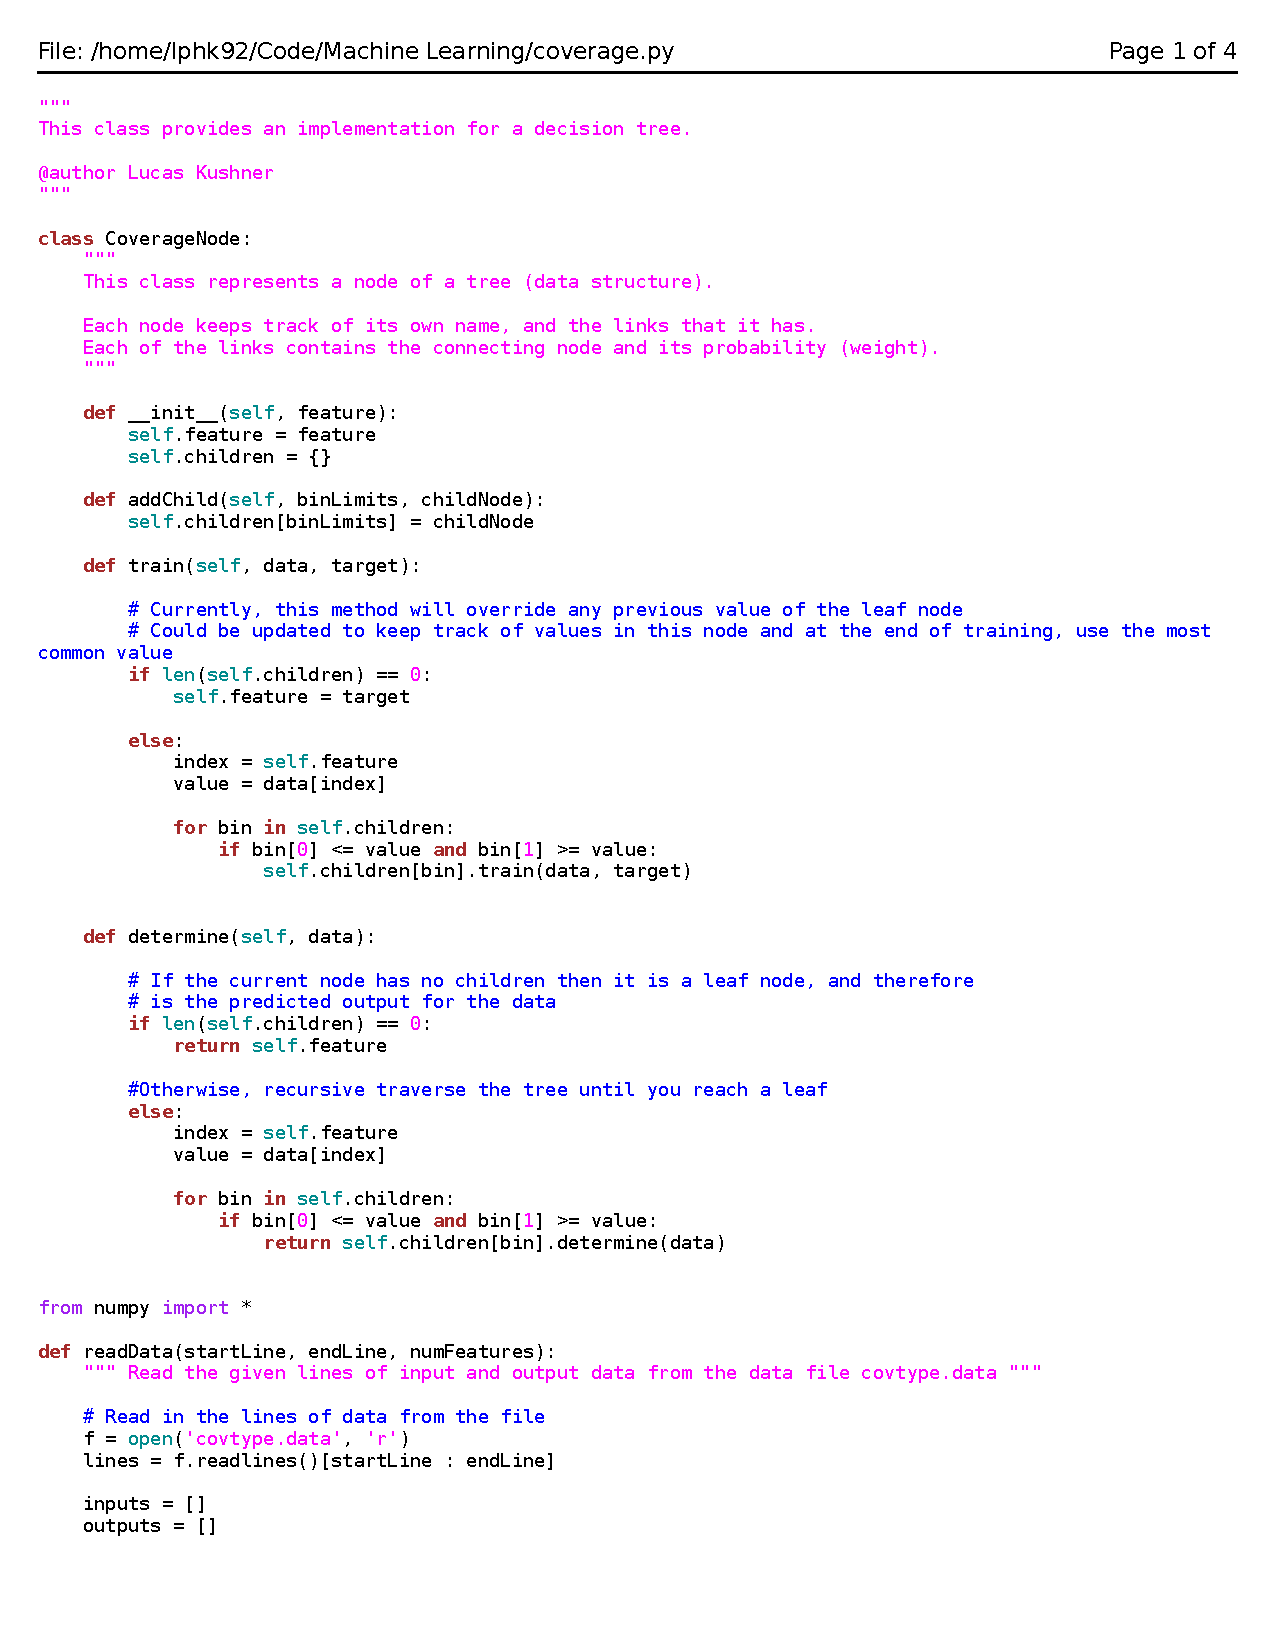
\includepdf[pages = 1-4]{coverage.pdf}
	
\end{document}
